\section{Parallelisierung der kritischen Abschnitte}

\subsection{Parallelisierung}
\begin{frame}{Verarbeitung einzelner Bildpaare}
	content...
\end{frame}

\begin{frame}{Innerhalb der Verarbeitung einzelner Bildpaare}
	\begin{figure}[h]
		\centering
		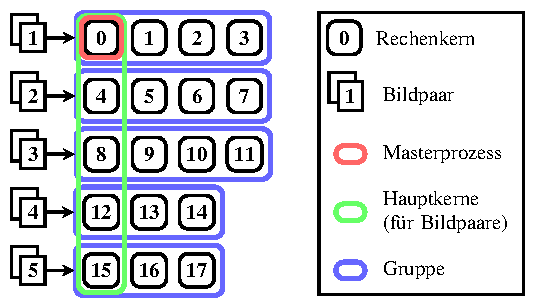
\includegraphics[width=0.5\textwidth]{pdf/parallel}
		\caption[Verteilung]{Verteilung von fünf Bildpaaren auf 18 Rechenknoten}
	\end{figure}
\end{frame}

\subsection{Optimierung der Performance-Engpässe in Python}
\begin{frame}[allowframebreaks]{Nutzen bereits optimierter Funktionen}
	content...
\end{frame}

\begin{frame}[allowframebreaks]{Kompilieren - Gesamtes Programm}
	asdf
\end{frame}

\begin{frame}[allowframebreaks]{Kompilieren - numba}
	asdf
\end{frame}

\begin{frame}[allowframebreaks]{Kompilieren - Cython}
	asdf
\end{frame}